% Created 2018-08-27 Mon 08:22
% Intended LaTeX compiler: pdflatex
\documentclass[presentation]{beamer}
\usepackage[utf8]{inputenc}
\usepackage[T1]{fontenc}
\usepackage{graphicx}
\usepackage{grffile}
\usepackage{longtable}
\usepackage{wrapfig}
\usepackage{rotating}
\usepackage[normalem]{ulem}
\usepackage{amsmath}
\usepackage{textcomp}
\usepackage{amssymb}
\usepackage{capt-of}
\usepackage{natbib}
\usepackage[linktocpage,pdfstartview=FitH,colorlinks,
linkcolor=blue,anchorcolor=blue,
citecolor=blue,filecolor=blue,menucolor=blue,urlcolor=blue]{hyperref}
\setbeamertemplate{frame footer}{\insertshortauthor}
\setbeamerfont{page number in head/foot}{size=\tiny}
\setbeamercolor{footline}{fg=gray}
\author{Florian Hollenbach}
\usepackage[english]{isodate}
\usepackage{amsmath,amsthm,amssymb,amsfonts}
\usetheme{metropolis}
\usecolortheme{}
\usefonttheme{}
\useinnertheme{}
\useoutertheme{}
\author{Florian Hollenbach}
\date{\today}
\title{Political Science 209 - Fall 2018}
\subtitle{Introduction}

\hypersetup{
 pdfauthor={Florian Hollenbach},
 pdftitle={Political Science 209 - Fall 2018},
 pdfkeywords={},
 pdfsubject={},
 pdfcreator={Emacs 25.3.1 (Org mode 9.1.9)}, 
 pdflang={English}}
\begin{document}

\maketitle


\begin{frame}[label={sec:org701effc}]{Introduction}
\begin{block}{Professor Florian Hollenbach}
\begin{itemize}
\item Ich bin ein Berliner
\item Masters from University of Potsdam
\item PhD in Political Science from Duke University
\item 2014/2015 Post-Doc at Princeton University
\item Assistant Professor in Political Science @ TAMU since Fall 2015
\item fhollenbach.org
\end{itemize}
\end{block}
\end{frame}


\begin{frame}[label={sec:orgd86d59f}]{Note Cards}
\begin{itemize}
\item Name

\item Where are you from? City, State, (Country)

\item How many people live where you are from?

\item What is something weird/interesting about you?

\item How can I help you learn better?
\end{itemize}
\end{frame}

\begin{frame}[label={sec:org0498c82}]{Note Cards}
\begin{itemize}
\item Name: Florian Hollenbach

\item Where are you from? City, State, (Country): Berlin, Germany

\item How many people live where you are from? 3.5 million

\item What is something weird and interesting about you? I randomly sing or whistle one line of a song over and over again

\item How can I help you learn better?  --
\end{itemize}
\end{frame}

\begin{frame}[label={sec:org17b2169}]{Introduction}
What do you think this class is (or should be) about?
\end{frame}


\begin{frame}[label={sec:orge0802cb}]{What is this class about?}
\begin{itemize}
\item How to do (political) science
\item How to read and understand (political) science
\item Programming in R
\item How does science work
\item Understand the world around you!
\end{itemize}
\end{frame}

\begin{frame}[label={sec:orgf903823}]{What is political science?}
\begin{itemize}
\item The study of politics
\item “scientific study of political phenomena”
\item Answer general phenomenon, not particular situations
\item More similar to economics than philosophy
\end{itemize}
\end{frame}

\begin{frame}[label={sec:orgcbbbec0}]{What is this class about?}
\begin{figure}[htbp]
\centering
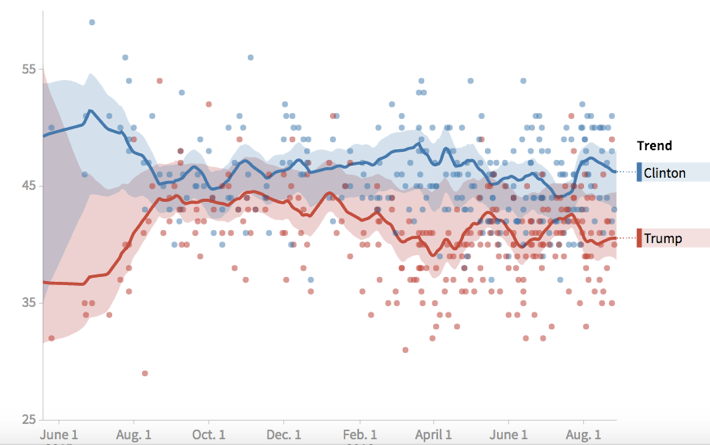
\includegraphics[width=.9\linewidth]{/Users/florianhollenbach/Documents/GitHub/Polisci209_2018/slides/week1/surveys.png}
\label{fig:org4e68d9c}
\end{figure}
\end{frame}

\begin{frame}[label={sec:org486fde4}]{What is this class about?}
\begin{figure}[htbp]
\centering
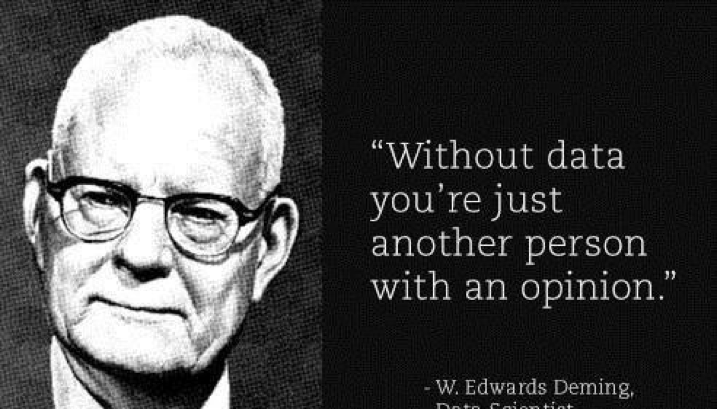
\includegraphics[width=.9\linewidth]{/Users/florianhollenbach/Documents/GitHub/Polisci209_2018/slides/week1/data_opinion.png}
\label{fig:org2d3e519}
\end{figure}
\end{frame}


\begin{frame}[label={sec:orgefef936}]{What is this class about?}
``Two transformative technological changes have driven this rapid growth of quantitative social science. First, the Internet has greatly facilitated data revolution, a spike in the amount and diversity of available data, through information sharing, making it possible for researchers and organizations to disseminate numerous data sets in digital form. Second, the computational revolution, in terms of both software and hardware, means that essentially anyone can conduct data analysis using their personal computer and favorite data analysis software without needing to access expensive computational facilities.'' -- Kosuke Imai
\end{frame}

\begin{frame}[label={sec:org9d24507}]{Class Resources}
Website: \url{https://fhollenbach.github.io/Polisci209\_2018/}
Syllabus: \url{https://fhollenbach.github.io/Polisci209\_2018/pages/syllabus.html}

eCampus \uline{\uline{only for submitting homework and posting grades}}
\end{frame}

\begin{frame}[label={sec:orgf55da46}]{Syllabus}
\url{https://fhollenbach.github.io/Polisci209\_2018/pages/syllabus.html}
\end{frame}


\begin{frame}[label={sec:org866cfc8}]{R and R-studio}
Please download and install r-studio on your computer:
\url{https://www.rstudio.com/products/rstudio/download/}
\end{frame}

\begin{frame}[label={sec:org4331190}]{Class Sessions}
\begin{itemize}
\item We will use R-Studio (or R) a lot in this class
\item This class will be very hard, but also rewarding
\end{itemize}

\begin{alertblock}{It is important that you do not get behind!}
Ask questions! Come to office hours (TA or myself) if you have trouble
\end{alertblock}
\end{frame}

\begin{frame}[label={sec:orgff4c814}]{Class Sessions}
\begin{itemize}
\item Lot's of exercises, few lectures
\item This requires that you do the readings and work through examples
\end{itemize}

\begin{alertblock}{Together we can make this class a lot of fun}
\end{alertblock}
\end{frame}


\begin{frame}[label={sec:org6611d36}]{R-Studio}
Hadley Wickham:
\begin{center}
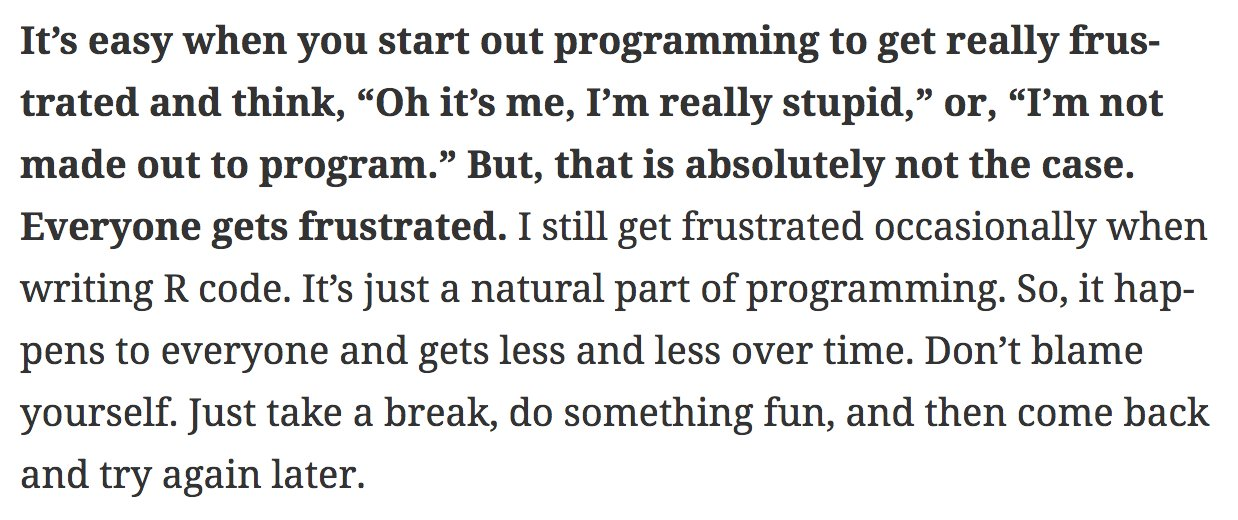
\includegraphics[width=9cm]{/Users/florianhollenbach/Documents/GitHub/Polisci209_2018/slides/week1/wickham.jpeg}
\end{center}
\end{frame}

\begin{frame}[label={sec:org6cc33eb}]{Create a folder for your class work}
\begin{center}
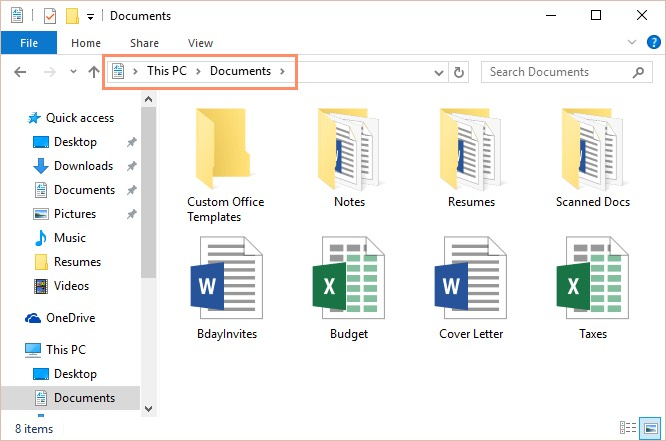
\includegraphics[width=5cm]{/Users/florianhollenbach/Documents/GitHub/Polisci209_2018/slides/week1/windowsfolder.jpeg}
\end{center}

\begin{center}
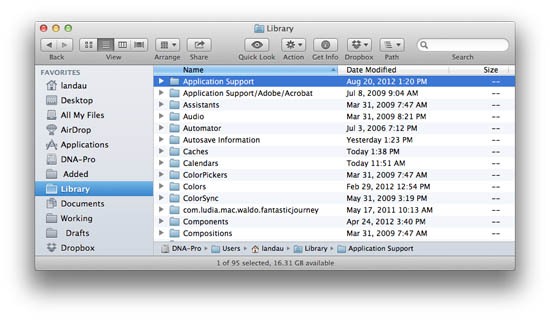
\includegraphics[width=5cm]{/Users/florianhollenbach/Documents/GitHub/Polisci209_2018/slides/week1/macfolder.jpeg}
\end{center}
\end{frame}

\begin{frame}[label={sec:orga7f3c7d}]{Create a folder for your class work}
\begin{itemize}
\item Go to the directory in which you want to create the folder in Finder/My Computer
\item Right click and select ``New Folder'' or press Shift-Command-N (Mac) / Ctrl+Shift+N (Win)
\item Name folder: ``Polisci209''
\end{itemize}
\end{frame}

\begin{frame}[fragile,label={sec:orgac30e63}]{Path}
 A path points to a file system location by following the directory tree hierarchy expressed in a string of characters in which path components, separated by a delimiting character, represent each directory

example
\begin{enumerate}
\item Mac:
\end{enumerate}
\begin{verbatim}
 /Users/florianhollenbach/Documents/Polisci209/
\end{verbatim}
\begin{enumerate}
\item Win:
\end{enumerate}
\begin{verbatim}
C:\Users\florianhollenbach\Desktop\Polisci209\
\end{verbatim}
\end{frame}


\begin{frame}[label={sec:org90f0dde}]{Path}
\begin{itemize}
\item On Mac you can find the path to any folder by right clicking on the folder, clicking ``Get Info'', and then marking and copying the address behin ``Where''

\item In Windows you can right click to the right of the address in the address bar and select ``Copy Address''
\end{itemize}
\end{frame}


\begin{frame}[label={sec:org20e875a}]{Homework}
\begin{itemize}
\item Take survey if you haven't done so
\item Read Chapter 1
\item Try to install R-studio
\end{itemize}
\end{frame}
\end{document}